\documentclass[a4paper]{jpconf}
\usepackage{graphicx}
\begin{document}
\title{Streamlining CASTOR to manage the LHC data torrent}

\author{G. Lo Presti, X. Espinal Curull, E. Cano, B. Fiorini, A. Ieri, S. Murray, S. Ponce and E. Sindrilaru}

\address{CERN, 1211 Geneva 23, Switzerland}

\ead{giuseppe.lopresti@cern.ch}


\begin{abstract}
This contribution describes the evolution of the main CERN storage system, CASTOR, as it manages the bulk data stream of the LHC and other CERN experiments, achieving over 90 PB of stored data by the end of LHC Run 1.
This evolution was marked by the introduction of policies to optimize the tape sub-system throughput, going towards a cold storage system where data placement is managed by the experiments' production managers. More efficient tape migrations and recalls have been implemented and deployed where bulk meta-data operations greatly reduce the overhead due to small files. A repack facility is now integrated in the system and it has been enhanced in order to automate the repacking of several tens of petabytes, required in 2014 in order to prepare for the next LHC run. Finally the scheduling system has been evolved to integrate the internal monitoring.
To efficiently manage the service a solid monitoring infrastructure is required, able to analyze the logs produced by the different components (about 1 kHz of log messages). A new system has been developed and deployed, which uses a transport messaging layer provided by the CERN-IT Agile Infrastructure and exploits technologies including Hadoop and HBase. This enables efficient data mining by making use of MapReduce techniques, and real-time data aggregation and visualization.
The outlook for the future is also presented. Directions and possible evolution will be discussed in view of the restart of data taking activities.
\end{abstract}


\section{Introduction. The LHC Data Torrent}

With the end of LHC Run 1, the data storage at CERN has marked the milestone of 100 PB. The Physics data represent the vast majority of these data, following an exponential trend that has seen the size of the stored data doubling every 19 months during the past 10 years (Figure \ref{fig:stats}). In this paper the main Physics data storage system, CASTOR (CERN Advanced STORage manager, \cite{castor}) is presented, which holds about 92 PB as of October 2013. The first section illustrates the evolution of the system as it specializes towards a Tape Archive solution. The second section shows the recent developments focused to streamline  service operations. The third section describes the new monitoring infrastructure that has been developed to perform  both real-time analysis of the system and data mining to extract long term trends. Finally, the future evolution is discussed in the last section.

\begin{figure}[h]
\begin{center}
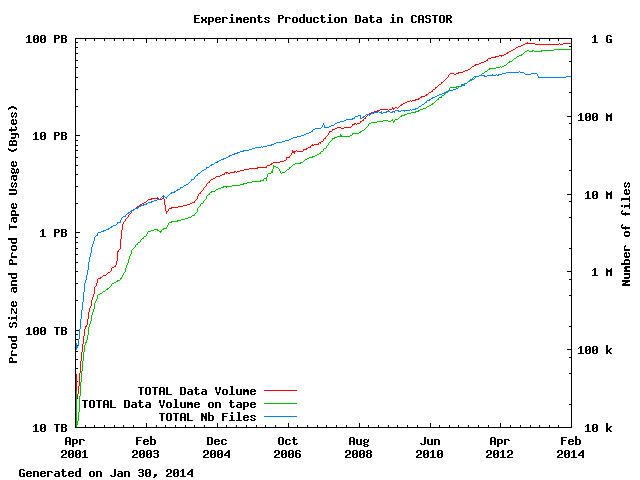
\includegraphics[width=28pc]{global_statistics.png}
\caption{\label{fig:stats}CASTOR usage over the past 10 years.}
\end{center}
\end{figure}

\section{Specialization}

Over the course of 2011 and 2012, the CASTOR service has addressed the Tier-0 data management requirements, focusing on a tape-backed storage solution, also known as the D0T1 ({\it Disk-0, Tape-1}) storage class. The primary goal has been to ensure smooth operations of the required experiments' work flows (data taking, reconstruction, export to other sites) as the experiments manage their data placement across the Storage Elements at the different sites.

Therefore, the development efforts focused on providing specific features and improvements. The scheduling system now integrates the resource monitoring, for a more dynamic and more reactive usage of the underlying disk resources. This has enabled the support of read-only hardware, where storage nodes that need some level of maintenance (e.g. rebuilding RAIDs) make their data available without being exposed to the extra load of write operations. Strong authentication has been introduced at the namespace level, thus ensuring data protection. Finally, expanding the scope of a Tape Archive solution a prototype for the CERN AFS backup has been put in place with minimal operational efforts: a pool of 17 storage nodes provides 290 TB of disk space, compared to a current backup volume in the order of 10 to 20 TB per day, and on the other side represents less than 3\% of the installed disk capacity for CASTOR. AFS at CERN \cite{dss} \cite{afs} has recently evolved into a much larger general-purpose file system, and its legacy TSM-based backup process shows its limits as the data volume increases. The new solution includes an encryption step at the AFS nodes, which have enough spare CPU cycles to encrypt the data on the fly, and a subsequent streaming to CASTOR, where the provided disk capacity ensures that backup operations terminate in the required time frame with a double copy on tape.

On the other hand, a consolidation effort has led to a significant simplification and reduction of the code base, as shown in Figure \ref{fig:loc}: with a release cycle of approximately one new release every 8 to 10 months, the last years have seen a consistent reduction in the number of C/C++ lines of code, whereas the figures for other languages did not increase significantly. This is justified both by the removal of legacy unused functionalities and by pushing the system business logic closer to the meta-data, or in other words by writing larger fractions of code in PL/SQL, thus fully exploiting the Oracle RDBMS engine CASTOR is based upon.

\begin{figure}[h]
\begin{center}
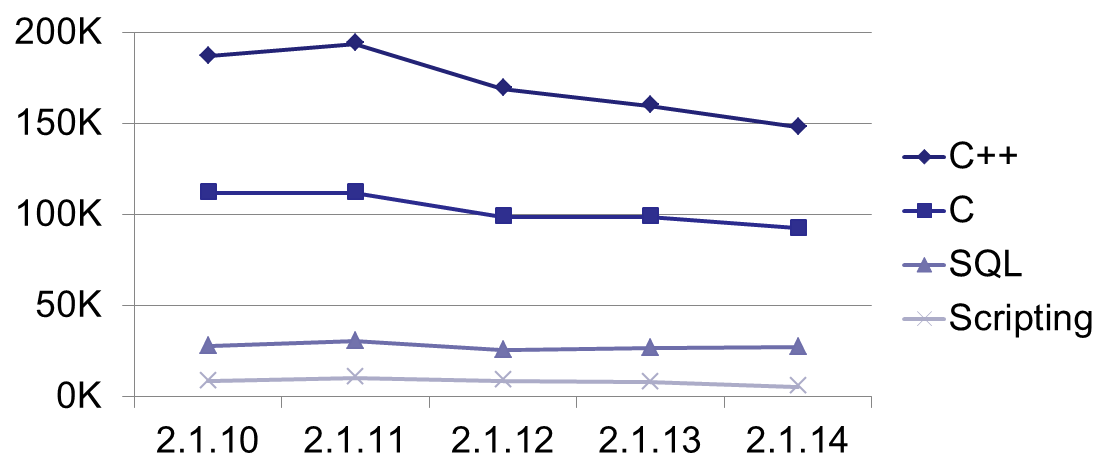
\includegraphics[width=23pc]{LoC_plot.png}
\hspace{1pc}%
\begin{minipage}[b]{12pc}
\caption{\label{fig:loc}Lines-of-code counts for the most recent CASTOR releases.}
\end{minipage}
\end{center}
\end{figure}


\section{Streamlining Operations}

As the main driver for new features has been the operations team, the CASTOR system has also evolved towards providing more maintainability and ultimately more dependability. The internal metadata processing has been redesigned in order to exploit bulk database interfaces. Now \textit{job} entities represent in the database any internal operation (e.g. replication of a disk copy to a different storage node, migration to tape, recall from tape). This had also the effect of lowering the per-file metadata overhead, which resulted in an increased overall throughput of the system. The system is now capable of sustaining 250 Hz of file write operations and 1 kHz of namespace operations compared to 120 Hz of file write operations of the previous version.

Finally, the system features a repacking facility, which has been improved with the addition of an independent tape queuing system in order to handle several hundreds of tapes in an unattended way. At CERN, repack operations \cite{repack} are run on a dedicated disk staging area, which includes approximately 830 TB of usable disk space. This facility is foreseen to be used in the upcoming months as a large repack campaign will take place, where some 100 PB of data will be migrated to new media, requiring a steady 3.8 GB/s throughput in order to complete the migration prior to the restart of the data taking activities.


\section{Monitoring}

To efficiently manage the service, a solid monitoring infrastructure is required. The new monitoring infrastructure of CASTOR is mainly based on log message analysis. This was made possible by the improvements of the different components of the system, so that they can report every action to their respective log files. Subsequently, a transport layer was deployed in order to ship these messages to different systems: the {\it LogViewer} to browse in real time the log records, the {\it Metric Analysis Engine} and the {\it Cockpit} to compute a set of metrics in real time over the flow of log messages, and finally an Hadoop FS is used to archive and enable data mining.


\subsection{Transport}

Every CASTOR component produces its own log files. These files are distributed (not evenly) in all the machines that are part of a CASTOR cluster. The first challenge of the new monitoring infrastructure was to transport these log files:
\begin{itemize}
\item efficiently, to be able to follow the high production rate and minimize the footprint and the extra resources needed (operation and hardware)
\item quickly, to enable real-time analysis
\item reliably, to prevent the loss of any message
\item modularly, to be able to easily replace any block of the transport sub-system in the future
\end{itemize}
These requirements were fulfilled with a modular architecture proposed by the team maintaining the messaging brokers of the CERN IT department, as can be seen in Figure \ref{fig:arch}.
A generic producer, named \texttt{simple-log-producer}, takes care of reading the different log files as they are written, similarly to the \texttt{tail} Unix command. Each line is considered as a unique and independent log record, which is then sent to the transport layer brokers using the STOMP protocol.
The multiple Apache ActiveMQ brokers deployed in the IT department are running behind a DNS alias, to bring high availability and load balancing. Here we \textit{produce to any, consume from all}. So the producers just need to send their messages to any broker behind the alias. However, the consumers need to consume from all the brokers. This is achieved by using a dynamic configuration file, which is updated each time a broker appears or disappears in the alias.

\begin{figure}[h]
\begin{center}
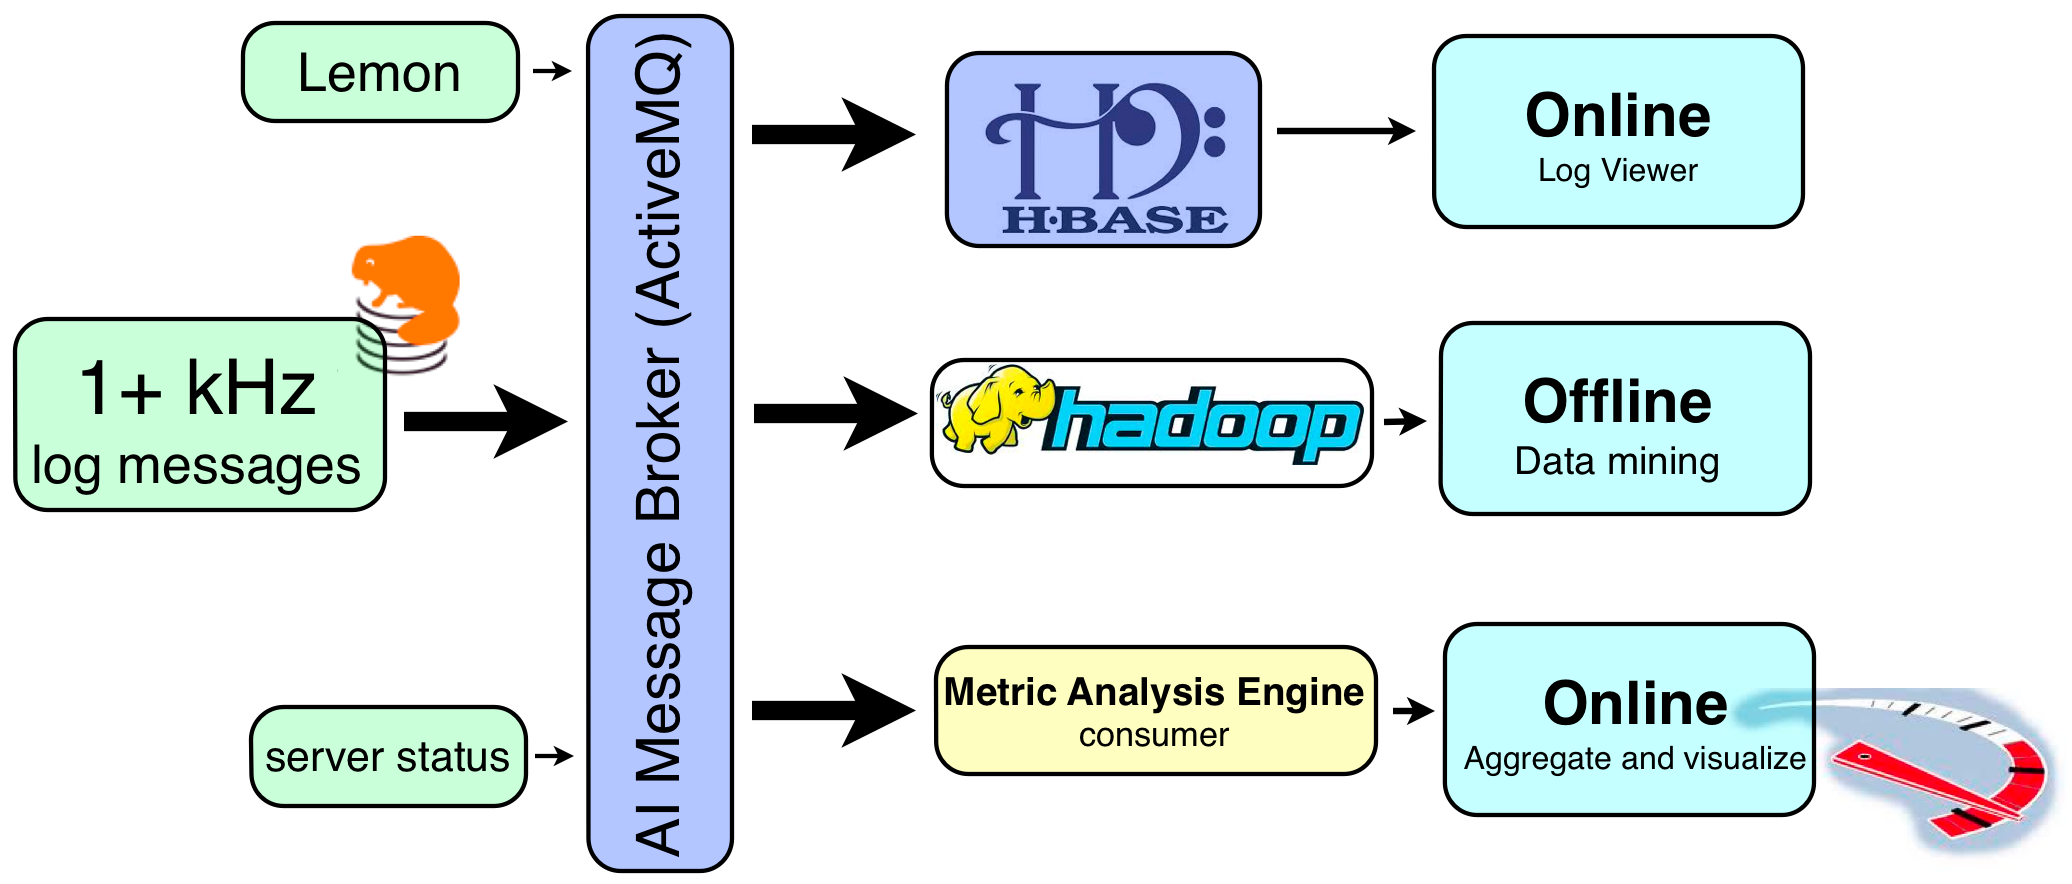
\includegraphics[width=32pc]{monitoring_architecture.png}
\caption{\label{fig:arch}The Monitoring architecture, with the IT Agile Infrastructure Message Broker and the components developed around it.
Among the inputs, Lemon [LHC Era Monitoring] provides basic hardware monitoring, and the CASTOR aggregated logs represent the bulk of the load at over 1 kHz rate.}
\end{center}
\end{figure}


\subsection{The LogViewer}

A tool to browse the log records is crucial for the developers and the operators of the service in order to debug and investigate operational issues. To meet this need, a simple consumer was developed. Its role is to insert the records in a column oriented database, \textit{Apache HBase}.
To determine the best schema, the query patterns were carefully analysed. It appeared that the logs needed to be queried by only three keys:
\begin{itemize}
\item file ID, to look into whole history of a file
\item request ID, to look into the history of a request
\item tape ID, to study the whole life of a tape
\end{itemize}
Therefore, after testing, it was decided to use these three keys as a HBase object key, and store the entire raw messages in the columns. Hence it is trivial to retrieve the entire set of required messages with a single query by object key. In a real-life example, the system returned nearly 180,000 records in 16.7 seconds, which compares well with traditional SQL-based technologies.

A Django web application was developed, in order to easily browse the HBase database: it allows querying by any of the three keys, and displays the list of corresponding log messages.


\subsection{The Metric Analysis Engine and the Cockpit}

The Metric Analysis Engine (MAE) is a framework designed to compute a set of metrics from the flow of messages. The input is a Python dictionary, and the output is another Python dictionary with computed values, aggregated as defined in a metric definition file. The following code describes a metric which counts the number of error message, over a 60 second sliding window using 3 bins. The results are also broken down by instance and daemon.
\scriptsize
\begin{verbatim}
<metric>
    name: Errors
    window: 60
    conditions: LVL == "Error"
    groupbykeys: INSTANCE, DAEMON
    data: Counter(COUNT)
    nbins: 3
</metric>
\end{verbatim}
\normalsize

A consumer for the transport layer was developed using the MAE framework. This component has two other roles: feeding a Django web application (the Cockpit) with the computed metric values, and making the computed metric values available via an RPC interface.

The Cockpit is capable of plotting and displaying the different metrics computed by the MAE in time series charts or histograms, as shown in Figure \ref{fig:scr}. It receives the metrics data via a REST (Representational State Transfer) interface, and stores the samples in a MySQL database.


\subsection{The HDFS Archive}

The last consumer component is responsible for archiving the log messages in the Hadoop Distributed File System (HDFS). The two main goals of this archive are the long term storage of the logs in an independent file system, and the ability to execute data mining analyses by means of the Hadoop \textit{MapReduce} framework.

Log messages are stored in this archive using the following hierarchy: the first level is the cluster name, e.g. \texttt{castorpublic}, the second level is the node type (head node or storage node), and the third level is the date. The consumer processes aggregate the messages before sending them to HDFS. Afterwards, MapReduce jobs are run to aggregate and merge the small files into larger chunks, more suitable for storing in HDFS.

This archive enables operators to run specialized data-mining analysis by writing simple MapReduce jobs to be run on Hadoop, thus exploiting the parallelism and data locality offered by the system. For instance, a typical activity is to run a trend analysis on a particular log message. On a traditional file-based store this would require executing multiple \texttt{grep}-like operations on several files scattered in different machines, and then aggregating the results by hand. The Hadoop streaming interface allows writing simple scripts for the Map and Reduce phases, and the interface takes care of running jobs to collect all aggregated results in one go at the end of their execution.

\begin{figure}[h]
\begin{center}
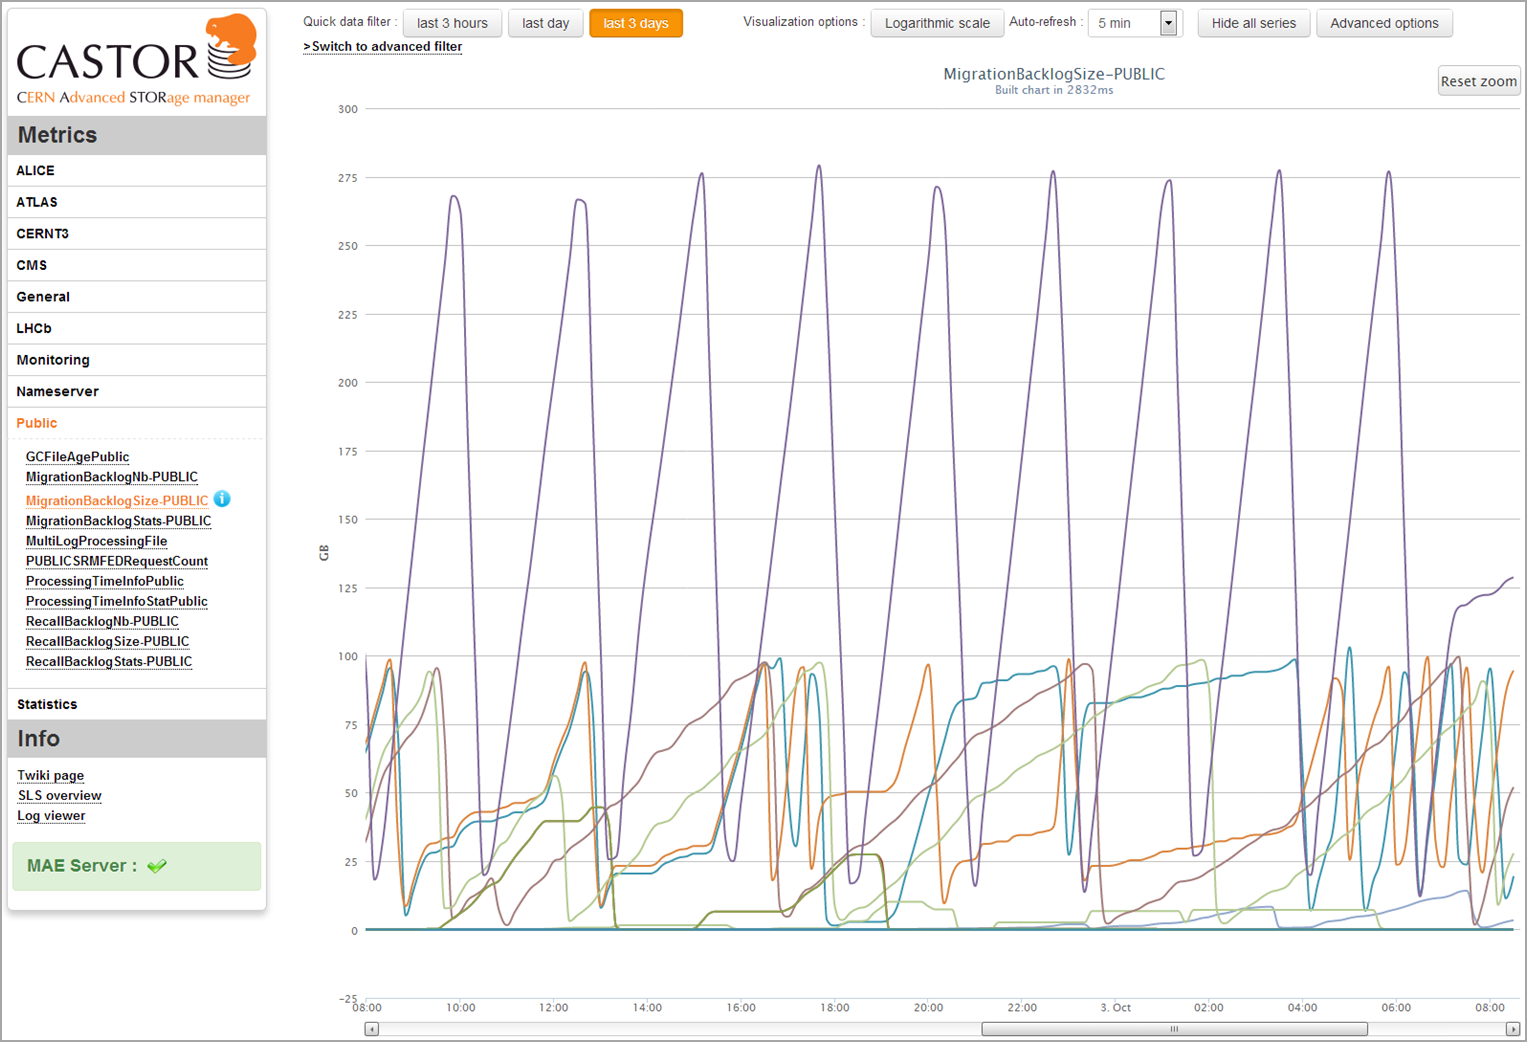
\includegraphics[width=36pc]{cockpit_screenshot.png}
\caption{\label{fig:scr}An illustrative screenshot of the Cockpit interface, showing for instance the migration-to-tape queue during 24 hours for the \texttt{castorpublic} cluster.}
\end{center}
\end{figure}



\section{Conclusions and Future Evolution}

In this paper, the CASTOR system and its monitoring infrastructure have been described. Its evolution to being predominantly a tape archive storage solution has been shown, and will clearly identify the role of the CASTOR service during the LHC Run 2.

A further simplification of the CASTOR system is foreseen. Among the currently supported protocols, RFIO, Root, GridFTP, and XRoot, the latter will take the role of the main native protocol instead of RFIO, while Root is about to be deprecated. GridFTP is gradually taken over by XRoot for the WAN transfers. The adoption of XRoot as the main file transfer protocol opens the possibility to exploit its upcoming features, including for instance the support of XRoot federations or the support of the HTTP protocol.
On the other side, only few disk pools for each experiment would serve as staging areas for the Tier-0 work flow, thus allowing for further streamlining operational procedures.

Finally, with the scaling of the storage nodes managed by the system, where larger and larger nodes providing nearly 100 TB of raw capacity are the building blocks of all storage systems, different hardware configurations are being considered to overcome the known limitations of RAID-0 configurations \cite{dss}. For instance, a foundation object-store-based layer may serve as a raw distributed storage, on top of which different storage services provide their specific features. To this end, \textit{Ceph} \cite{ceph} is being investigated as a possible solution for a disk backend for CASTOR, with the aim of disentangling low level disk operations from the service operations. Other services are expected to follow, with the aim to provide a consistent layered services architecture.


\section*{References}

\begin{thebibliography}{5}
\bibitem{castor} The CASTOR web site, \textit{http://cern.ch/castor}
\bibitem{dss} Espinal X et al., \textit{Disk storage at CERN: handling LHC data and beyond}, CHEP 2013, Amsterdam
\bibitem{afs} Van der Ster D et al., \textit{Toward a petabyte-scale AFS service at CERN}, CHEP 2013, Amsterdam
\bibitem{repack} Kruse D F, \textit{The Repack Challenge}, CHEP 2013, Amsterdam
\bibitem{ceph} Van der Ster D et al., \textit{Building an organic block storage service at CERN with Ceph}, CHEP 2013, Amsterdam
\end{thebibliography}


\end{document}
